\section{Measuring the learnability of congestion control}
\label{s:operational}

We conducted an experimental study to examine several aspects of
congestion-control learnability, by using Remy as an instrument to ask
questions of the form: how faithfully do protocol designers really
need to understand the networks they design for? What knowledge about
the network is important to capture in a design process, and what
simplifications are acceptable?

\subsection{Knowledge of network parameters}

\label{s:oprangeperftradeoff}

We evaluated the difficulty of designing a congestion-control
protocol, subject to imperfect knowledge about the parameters of the
network.

Some congestion-control protocols have been designed for specific
kinds of networks~\cite{dctcp,westwood} or require explicit knowledge
of the link rate \emph{a priori}~\cite{xcp}. Others are intended as a
``one size fits all,'' including most variants of TCP.

We set out to answer a question posed in~\cite{wroclawski}: are ``one
size fits all'' protocols inherently at a disadvantage, because of a
tradeoff between the ``operating range'' of a protocol and its performance?

To quantify this, we designed four RemyCCs for training
scenarios encompassing a thousand-fold variation in link rates, a
hundred-fold variation, a ten-fold variation, and a two-fold
variation. Each range was centered on the geometric mean of 1 and
1000~Mbps (32 Mbps), and each set of training scenarios sampled 100
link rates logarithmically from the range. The training scenarios are
shown in Table~\ref{table:oprange}.

\begin{table}
\caption{Training scenarios for ``knowledge of network parameters''
  experiment, showing the effect of varying the intended link rate
  operating range. Each RemyCC was designed for a network with a single
  bottleneck, and each sender with a mean ``on'' and ``off'' time of
  1~s.}
\label{table:oprange}
\begin{center}
\begin{tabular}{l|l|l|l}
\bf RemyCC & \bf Link rates & \bf RTT & \bf Max.~number of senders \\
\hline
1000x  & 1--1000~Mbps & 150~ms & 2 \\
100x   & 3.2--320~Mbps & 150~ms & 2 \\
10x    & 10--100~Mbps & 150~ms & 2 \\
2x     & 22--44~Mbps & 150~ms & 2 \\
\end{tabular}
\end{center}
\end{table}

We tested these schemes in ns-2 by sweeping the link speed between 1
and 1000~Mbps, keeping the other details of the simulated network
identical to the training scenario. The results are shown Figure~\ref{fig:breadth}.

\begin{figure}
%\begin{subfigure}[b]{0.49\textwidth}
%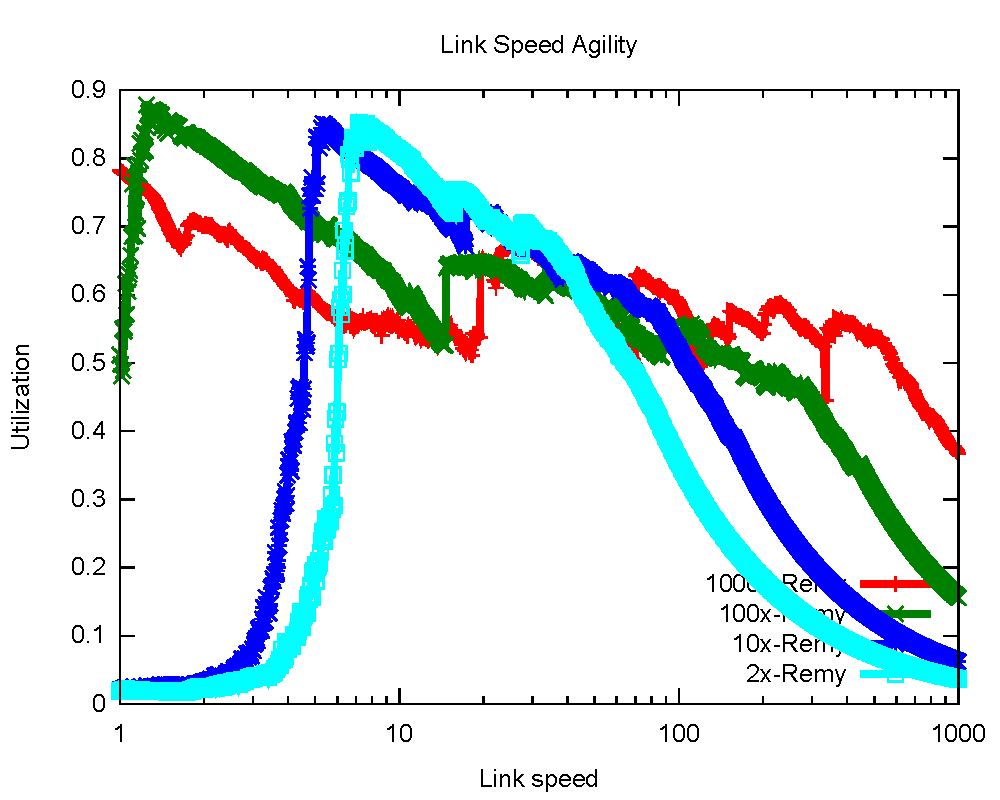
\includegraphics[width=\textwidth]{tradeoff-tpt.pdf}
%\end{subfigure}
%\begin{subfigure}[b]{0.33\textwidth}
%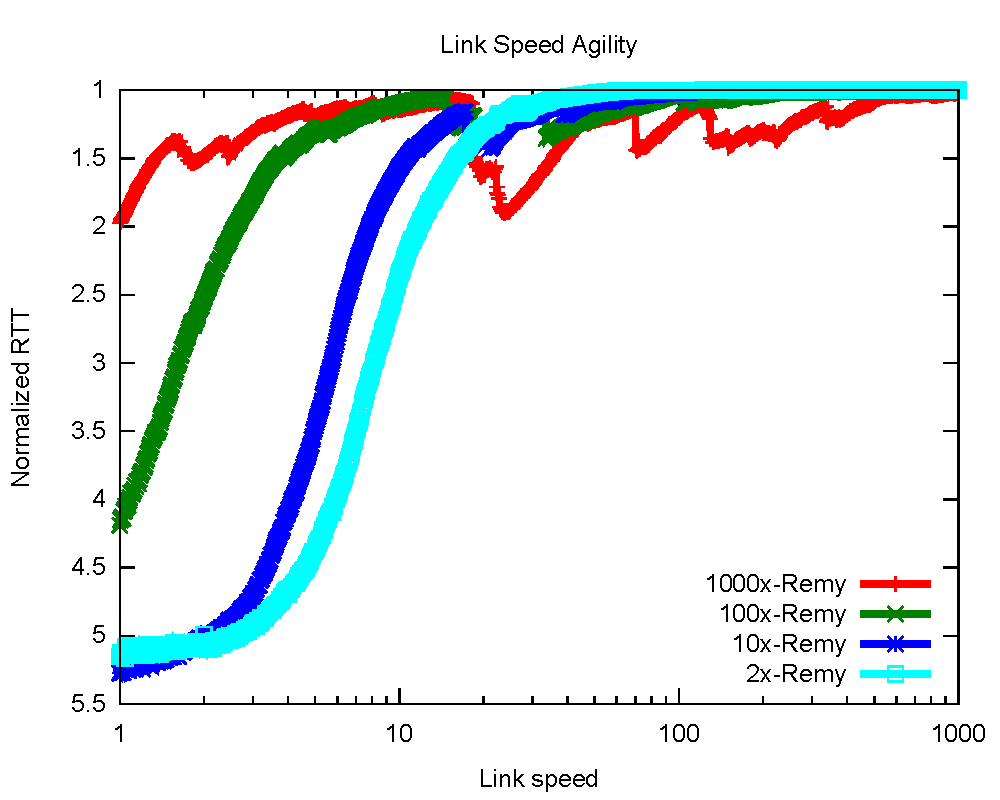
\includegraphics[width=\textwidth]{tradeoff-delay.pdf}
%\end{subfigure}
%\begin{subfigure}[b]{0.49\textwidth}
%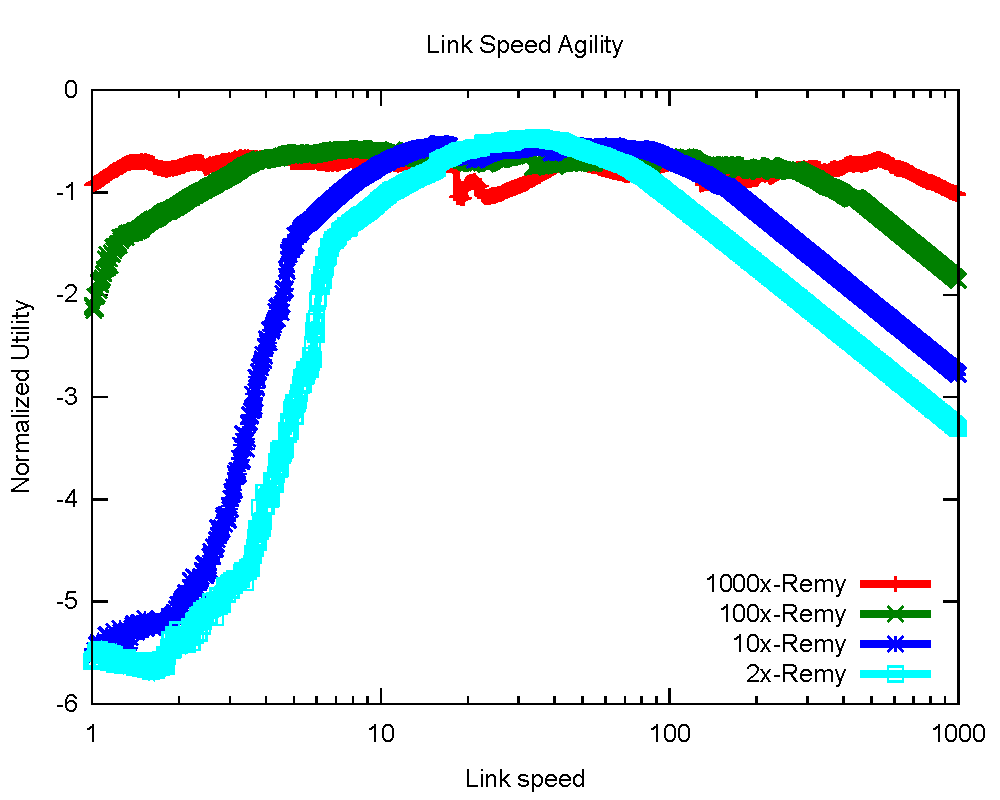
\includegraphics[width=\textwidth]{tradeoff-util.pdf}
%\end{subfigure}
\caption{Evidence of a weak tradeoff between operating range of a
  congestion-control protocol and performance. The RemyCC protocols
  designed with more specific network models (RemyCC-2x and RemyCC-10x)
  performed modestly better---within their design ranges---than protocols
  designed for a broader range of networks (RemyCC-100x and RemyCC-1000x),
  at a cost of deterioration when the actual network did not fall
  within the training scenarios. The four RemyCC protocols outperformed
  Cubic and Cubic-over-sfqCoDel over their respective design ranges.}
\label{fig:breadth}
\begin{center}
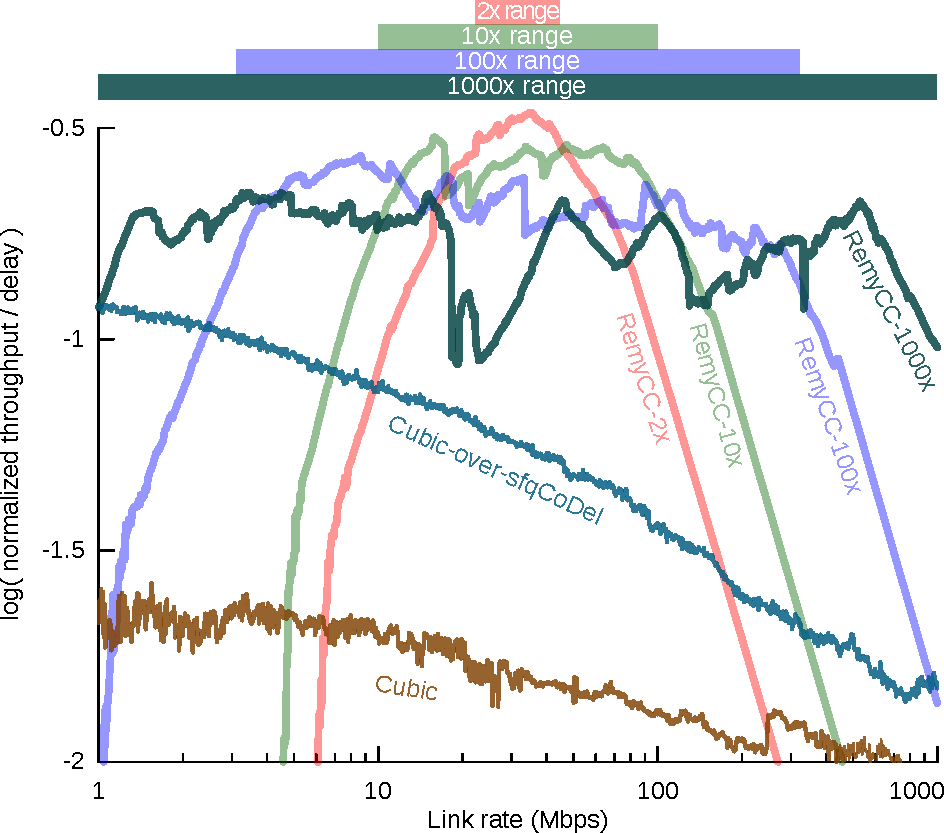
\includegraphics[width=\columnwidth]{oprange-manual.pdf}
\end{center}
\end{figure}

We found only weak evidence of a tradeoff between operating range and
performance: optimizing for a smaller range did help modestly within
that range. Because of the small magnitude of the effect, we cannot
say for sure whether simply spending more time optimizing the
broader-score RemyCCs might bring their performance closer to the
narrower-scope RemyCCs. Each RemyCC outperformed the human-designed
algorithms over its full design range, suggesting that it may be
possible to construct ``one size fits all'' RemyCCs that outperform
TCP across a broad range of real-world conditions, even when TCP is
assisted by in-network algorithms.

\subsection{Structural knowledge}
\label{ss:topological}

\begin{figure}
\caption{Parking-lot topology used to measure the consequences of imperfect
knowledge about the network's structure.}
\label{fig:two-link}
\begin{center}
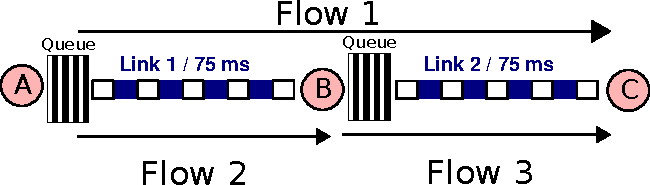
\includegraphics[width=\columnwidth]{twolink.pdf}
\end{center}
\end{figure}

We evaluated the difficulty of designing a congestion-control
protocol, subject to imperfect knowledge of the network's structure or
topology.

It is an understatement to say that the Internet is a vast network
whose full structure is known to nobody and which no model can
accurately capture. Nonetheless, researchers regularly develop new
distributed protocols for the Internet, which are deployed based on
tests in example network paths that imperfectly capture the Internet's
true complexity.

In practice, protocol designers expect that they can reason about the
performance of a distributed network algorithm by modeling the network
as something simpler than it is. We worked to capture that intuition
rigorously by studying quantitatively how difficult it is to learn a
congestion-control protocol for a more-complicated network, given a
simplified model of that network's structure.

In ns-2, we simulated a network with two bottlenecks in a
``parking-lot'' topology, shown in Figure~\ref{fig:two-link}. Flow 1
crosses both links and encounters both bottlenecks. It contends with
Flow 2 for access to the bottleneck queue and note A, and contends
with Flow 3 for access to the bottleneck queue at node B.

\begin{figure}[t!]
\caption{How well do endpoints need to understand the network around
  them? To assess this, we measure the throughput of three
  congestion-control schemes across a simulated two-hop network path,
  as the rate of each link is swept between 10 and 100~Mbps, with
  75~ms of delay per hop. A RemyCC designed for a simplified
  one-bottleneck model of the network performs 17\% worse, on average,
  than a RemyCC designed with knowledge of the network's true
  two-bottleneck structure. Both RemyCCs outperform TCP Cubic assisted
  by per-flow queueing and CoDel at the bottlenecks.}
\label{f:multihop}
\begin{center}
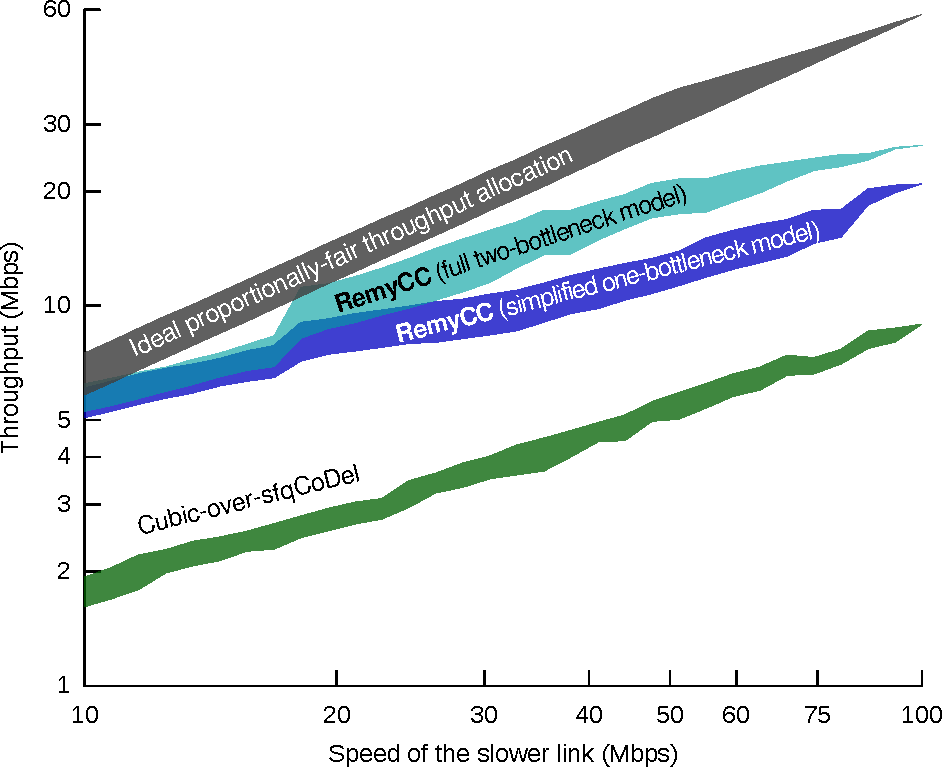
\includegraphics[width=\columnwidth]{multilink-all.pdf}
\end{center}
\end{figure}

The results for Flow 1 (the flow that crosses both links) are shown in
Figure~\ref{f:multihop}.\footnote{Results for Flow 2 and Flow 3
  (flows crossing only a single link) were nearly identical between
  the schemes.} The experiment sweeps the rate of each of the two
links between 10 and 100~Mbps, and the shaded area in the figure shows
the full locus of throughputs seen by Flow 1. For each pair of rates
(for link 1 and link 2), we also calculate the ideal
proportionally-fair throughput allocation, and plot the locus of these
points as well.

%Figure~\ref{f:multihop} shows the end-to-end throughput of connections
%traversing two bottleneck links for different protocols, including two
%RemyCCs. In each experiment, there were three flows: one that
%traversed two hops (the measured connection), a cross-traffic flow
%that traversed only the first bottleneck, and another cross-traffic
%flow that traversed only the second bottleneck.

%of two Tao protocols, running over a simulated two-hop network path
%and contending with cross traffic that runs over the first or
%second link only.

The RemyCC that was designed for the true network achieves close to
the ideal proportionally-fair throughput allocation across the two
links. The RemyCC that was designed for a simplified model of the
network with only one hop also performs adequately, but a little worse
than the ``true-network'' RemyCC. However, both computer-generated
protocols come closer to the ideal than contemporary protocols in wide
use, TCP Cubic~\cite{cubic}, the default TCP in Linux, running over
per-flow queueing and CoDel~\cite{CoDel}, an active queue management
(AQM) scheme that runs at both bottlenecks.

The results suggest that a congestion-control protocol designed for a
simplified model of the network's structure can experience a
quantifiable---but in this case modest---penalty to its performance.

\begin{table}
\caption{Training scenarios used to measure the consequences of imperfect
  knowledge of the network structure. Both protocols were designed for
  link rates distributed log-uniformly between 10 and 100~Mbps, and
  for flows with mean ``on'' and ``off'' time of 1~second.
}
\label{table:topology-training}
\begin{center}
\begin{tabular}{l|l|l}
\bf RemyCC & \bf Links modeled & \bf Num.~senders \\
\hline
one-bottleneck & one, 150~ms delay & 2 \\
true network & two, 75~ms delay each & 3 \\
\end{tabular}
\end{center}
\end{table}

\subsection{Knowledge about other endpoints}

\begin{comment}
\begin{figure*}[b!]
%\centering
%\begin{subfigure}[b]{\columnwidth}
%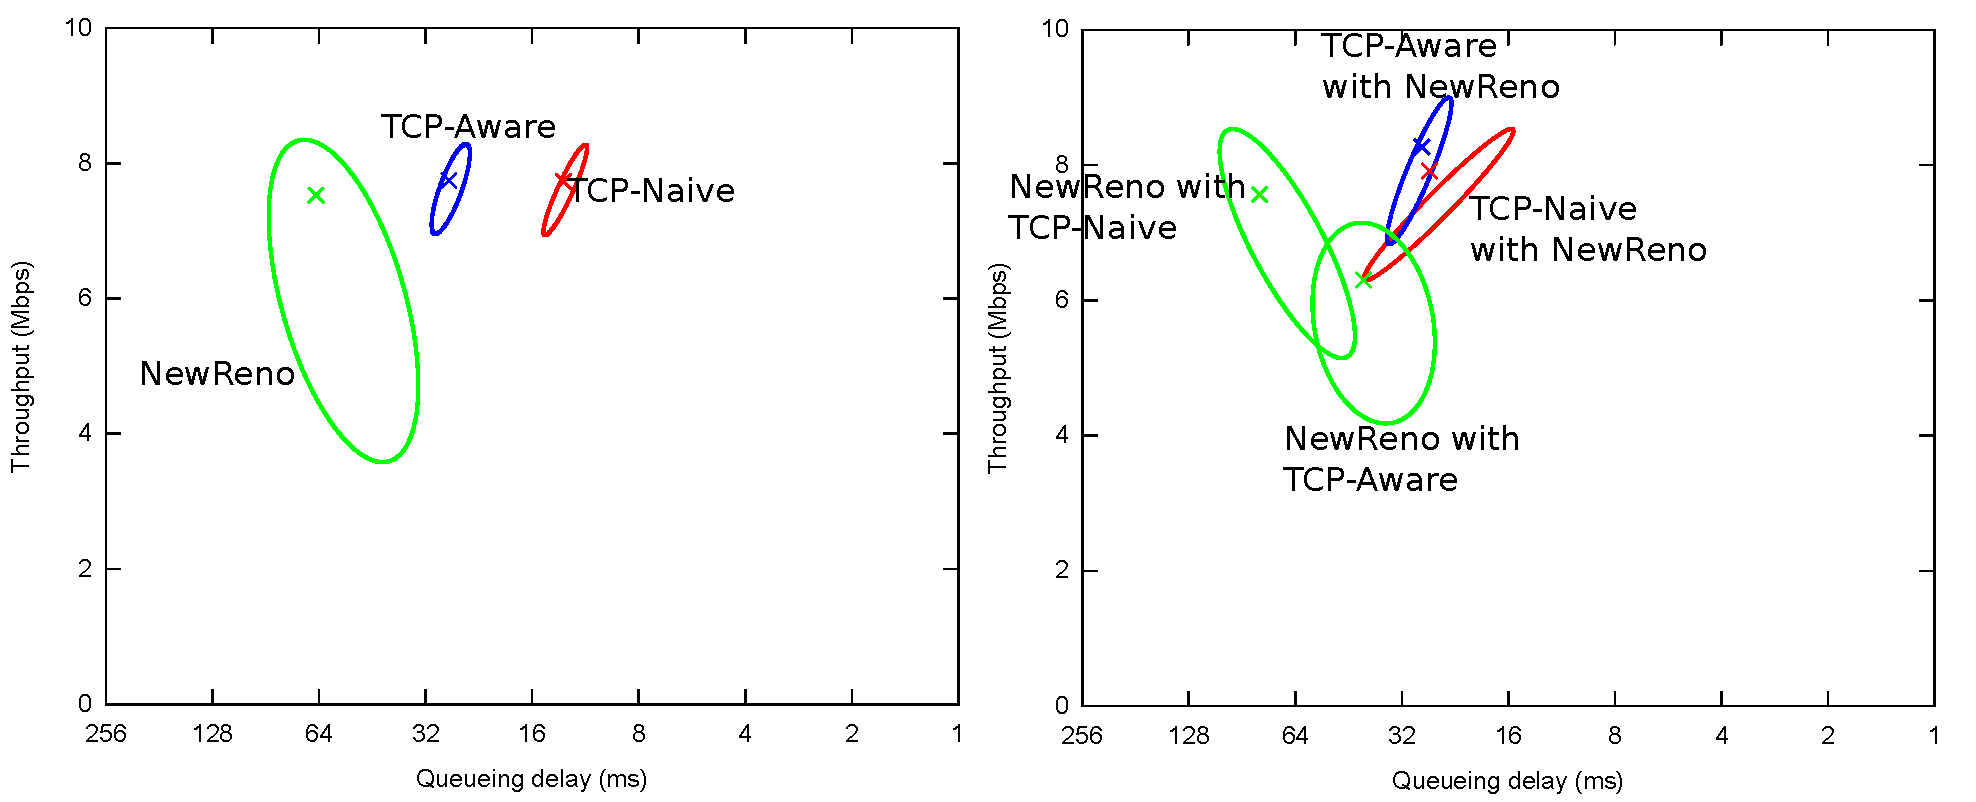
\includegraphics[width=\columnwidth]{compatible-5sec.pdf}
%\caption{TCP-Aware and TCP-Naive RemyCCs, 5 second ON/OFF}
%\end{subfigure}
%
%\begin{subfigure}[b]{\columnwidth}
\caption{RemyCCs designed with and without TCP-awareness,
  competing against themselves or against TCP. Shown here, two
  endpoints contending for a 10~Mbps link with 100~ms RTT, 250 kB of
  buffer capacity (200~ms maximum queueing delay), and
  almost-continuous offered load. The fair share of throughput is
  5~Mbps per endpoint. Ellipses show 1-$\sigma$ range of results.}
%\end{subfigure}
\label{fig:tcpaware}
\begin{center}
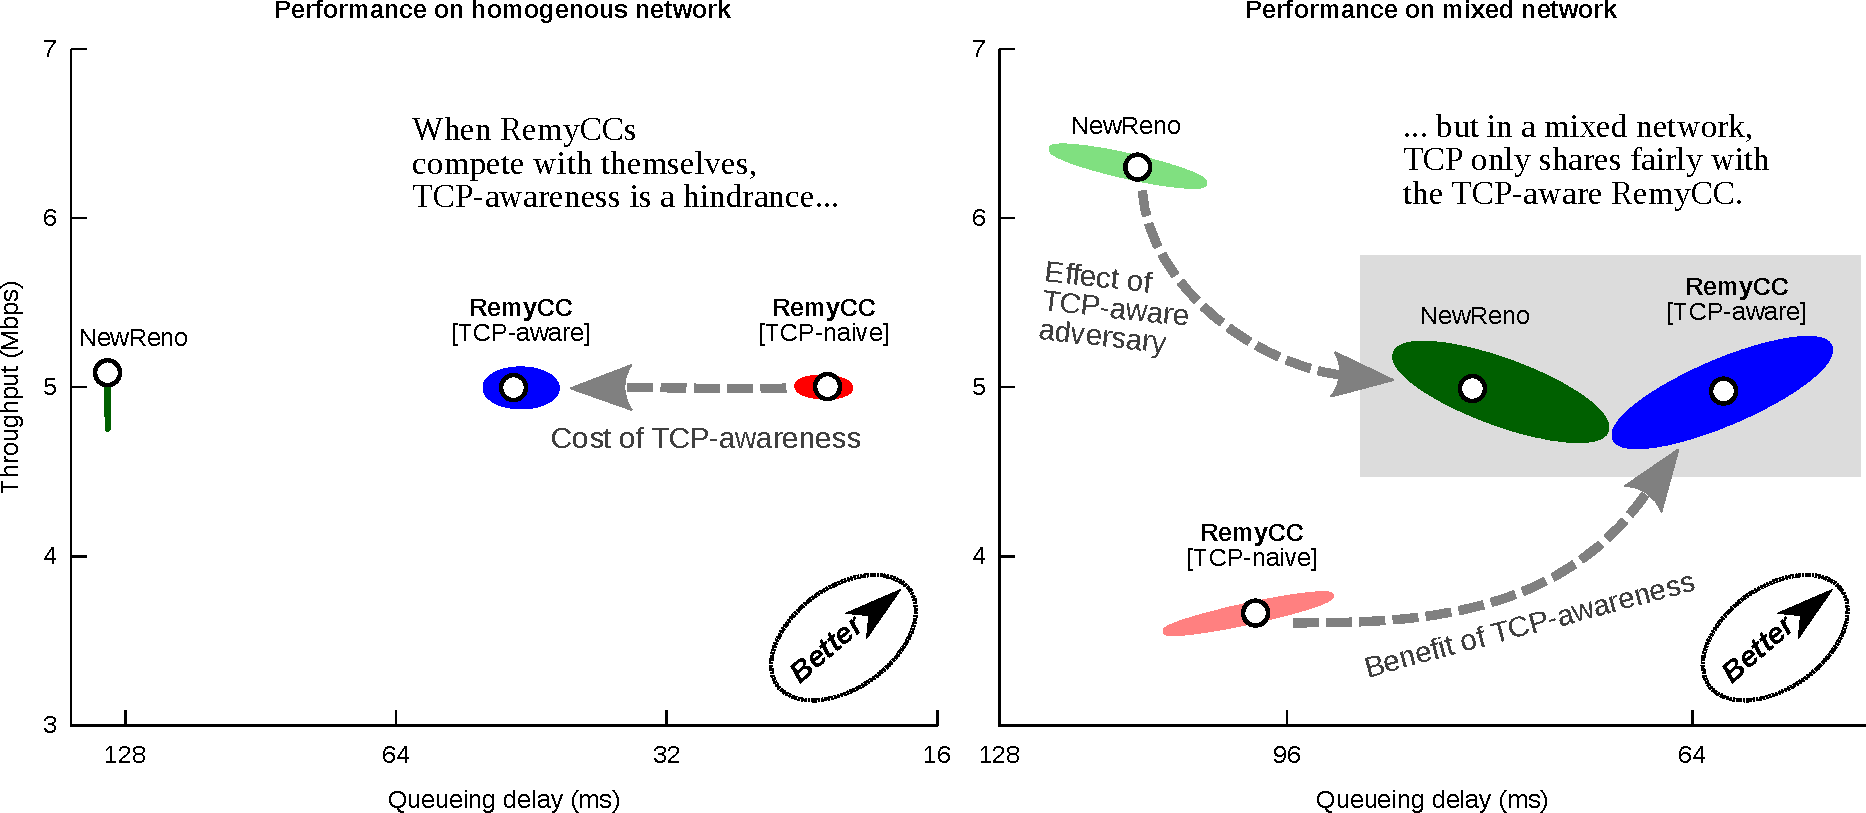
\includegraphics[width=\textwidth]{figures/manual/compatibility-drawn.pdf}
\end{center}
\end{figure*}
\end{comment}

\label{s:tcpaware}

We investigated the consequences of designing a congestion-control
protocol with the knowledge that some cross-traffic may the product of
pre-existing incumbent protocols.

This question has considerable practical relevance; in practice, the
developer of a new network protocol will rarely be able to arrange a
``flag day'' when all endpoints switch to the new
protocol.\footnote{There has not been a ``flag day'' on the Internet
  since the switch to IP in 1983.}

On the broad Internet today, cross-traffic will typically be the
product of traditional loss-triggered TCP congestion-control
protocols, such as NewReno or Cubic. This status quo presents a
serious problem for new protocols that seek to perform differently or
that try to avoid building up standing queues inside the network.

Some protocols, such as Vegas~\cite{vegas}, perform well when
contending only against other flows of their own kind, but are
``squeezed out'' by the more-aggressive cross-traffic produced by
traditional TCP. Conventional wisdom is that any ``delay-based''
protocol will meet a similar fate. This has contributed to a lack of
adoption of Vegas and other delay-based protocols.

Ideally, a newly-designed protocol would perform well (e.g.~high
throughput, low delay) when interacting with other endpoints running
the same protocol, \textbf{and} would appropriately share a network
with incumbent endpoints running traditional TCP. But what are the
consequences of building this ``TCP-awareness'' into a protocol?

We studied this by designing two network protocols for a simple
network---one whose model specified that the cross-traffic would be
from the same protocol, and one whose model included a training
scenario where the cross-traffic was from traditional TCP half the
time.

\begin{figure}
\caption{Performance of two flows of the same congestion-control
  scheme contending for a 10~Mbps link, for three different
  congestion-control schemes. The ``TCP-naive'' RemyCC is designed
  under the assumption that its competition, when present, is governed
  by the same RemyCC---an assumption that holds here. The
  ``TCP-aware'' RemyCC is designed under the assumption that its cross
  traffic has a 50\% chance of being governed by a TCP AIMD-like
  scheme. The results quantify the degree to which designing a
  protocol to play well with TCP can exact a cost when TCP is absent.}
\label{fig:tcphomog}
\begin{center}
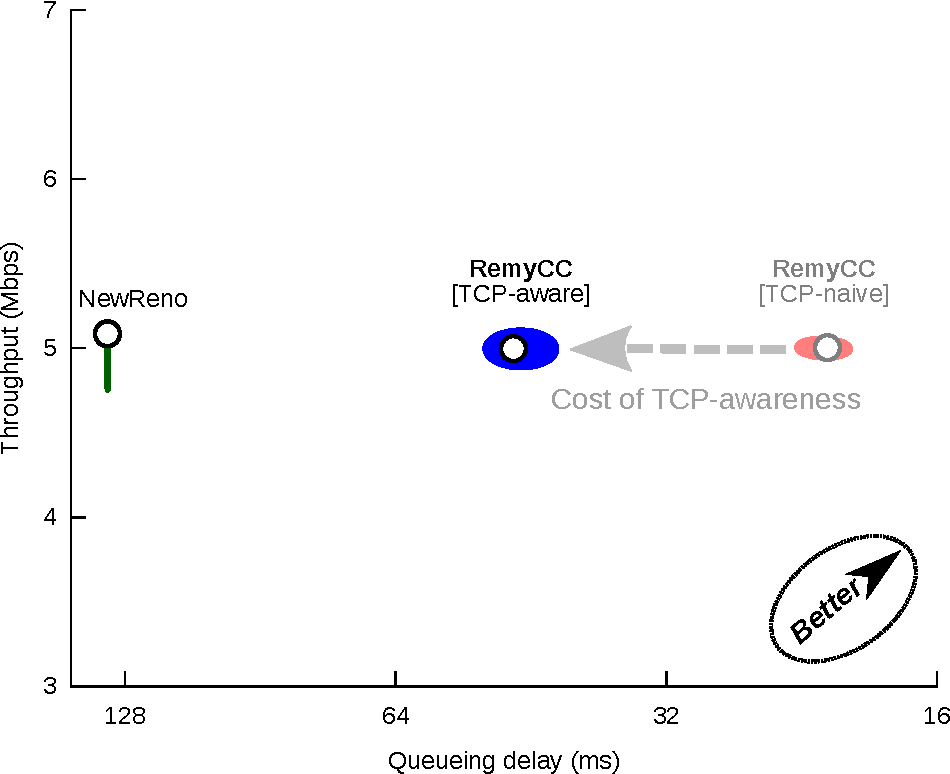
\includegraphics[width=\textwidth]{homo-3.pdf}
\end{center}
\end{figure}

\begin{figure}
\caption{When cross traffic is governed by TCP NewReno, the TCP-aware
  RemyCC achieves a more equitable division of the link---and better
  delay for both flows---than the TCP-naive RemyCC. The results
  demonstrate the benefit of TCP-awareness when TCP is present.}
\label{fig:tcpheterog}
\begin{center}
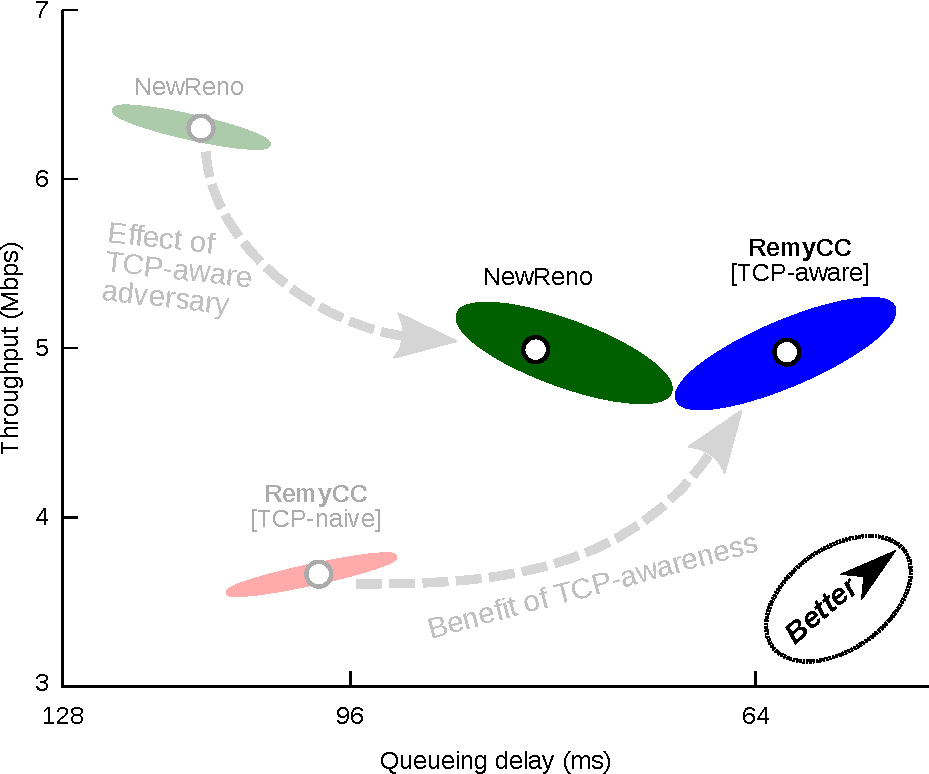
\includegraphics[width=\textwidth]{hetero-3.pdf}
\end{center}
\end{figure}

In Figure~\ref{fig:tcphomog}, protocols compete only with
cross-traffic from the same protocol. In this homogeneous setting,
adding TCP-awareness to a RemyCC builds up standing queues, more than
doubling the queueing delay without affecting throughput.

But in a mixed setting (Figure~\ref{fig:tcpheterog}) where a RemyCC
competes against TCP NewReno, the TCP-naive RemyCC is squeezed out and
does not get its fair share of the link. In the shaded region showing
the results when NewReno competes with the TCP-aware RemyCC,
TCP-awareness allows the RemyCC to claim its fair share of the link
and reduces the queueing delay experienced both by itself and by TCP
NewReno.

The results suggest that new delay-minded protocols \emph{can} avoid
being squeezed out by traditional loss-triggered TCP, but building in
this behavior comes at a cost to performance in the absence of TCP
cross-traffic.

